\documentclass[12pt]{article}

\usepackage{sbc-template}

\usepackage{graphicx,url}

\usepackage{amsmath}

%\usepackage[brazil]{babel}   
\usepackage[utf8]{inputenc}  
     
\sloppy

\title{Algoritmos de Segmentação de Imagem Baseados em Grafos}

\author{Fábio Antônio C. Andrade\inst{1}, Lucas A. Barros\inst{1}, Pedro M. Lima\inst{1}, Pedro R. Maia\inst{1} }

\address{Instituto de Ciências Exatas e Informática -- Pontifícia Universidade Católica de Minas Gerais
  \\Belo Horizonte -- MG -- Brasil
  \email{\{fabio.andrade.1452236, lucas.alkmim.1450684, pedro.lima.1463698, }
  \email{pedro.maia.1469860\}}@sga.pucminas.br}

\begin{document} 

\maketitle

\begin{abstract}
  This paper presents the implementation of two graph-based image segmentation algorithms proposed by \cite{Felzenszwalb2004} and \cite{boykov:06}. While Felzenszwalb-Huttenlocher performs segmentation based on regions and internal differences, Boykov--Funka-Lea models segmentation as energy minimization, using \textit{max-flow/min-cut} algorithms.
\end{abstract}
     
\begin{resumo} 
  Este artigo apresenta a implementação de dois algoritmos de segmentação de imagem baseados em grafos, propostos por \cite{Felzenszwalb2004} e \cite{boykov:06}. Enquanto Felzenszwalb-Huttenlocher realiza a segmentação a partir de regiões e diferenças internas, Boykov--Funka-Lea modela a segmentação como minimização de energia, utilizando algoritmos de \textit{max-flow/min-cut}.
\end{resumo}

\section{Introdução} \label{sec:intro}
O problema de segmentação de imagem é um grande desafio da visão computacional. Por ser um problema com uma alta gama de aplicações, como análise médica, reconhecimento de objetos, sistemas de navegação autônoma e processamento de vídeos, algoritmos que resolvam o problema são de extrema relevância.

Dentre os métodos existentes para a segmentação de imagem, existem aqueles baseados em grafos. Este trabalho foca em dois algoritmos desse tipo: o método de \cite{Felzenszwalb2004}, que busca identificar limites entre regiões com base na variabilidade local; o método de \cite{boykov:06} que formula o problema como uma minimização de energia.

Neste artigo, são apresentadas implementações de ambos os métodos e a aplicação deles em imagens reais e sintéticas.

\section{Trabalhos Relacionados} \label{sec:relatedwork}
A literatura utilizada como base para esse trabalho foram os artigos de \cite{Felzenszwalb2004} e \cite{boykov:06}.

\cite{Felzenszwalb2004} desenvolveram um algoritmo de segmentação de imagem baseado em um predicado para medir evidência para um limite entre duas regiões, considerando a variabilidade interna e as diferenças entre elas. Utilizando uma representação baseada em grafos para a imagem, cada pixel se torna um vértice, com as diferenças em relação as vizinhos se tornando arestas pesadas.

Apesar de ser baseado em decisões gulosas, o algoritmo produz segmentações que satisfazem propriedades globais. O artigo apresentou aplicação do algoritmo para dois tipos distintos de vizinhanças locais: grafos de grade e grafos de vizinhos próximos.

\cite{boykov:06} aborda métodos para segmentação de imagens com N dimensões utilizando cortes em grafos. Este trabalho apresenta algoritmos que exploram representações gráficas de imagens, onde os pixels ou voxels são modelados como nós de um grafo, e as relações entre eles (como similaridade de intensidade ou conectividade) são representadas como arestas com pesos. 

O método de cortes em grafos otimiza uma função de energia que combina termos de fidelidade aos dados (baseados na aparência dos pixels) e regularização (que incentiva bordas suaves na segmentação). O artigo destaca como essa abordagem pode ser aplicada eficientemente em imagens 2D e 3D, sendo útil em áreas como visão computacional e análise médica.

\section{Algoritmos e Implementação} \label{sec:algorithms}
Os algoritmos propostos por \cite{Felzenszwalb2004} e \cite{boykov:06}, mencionados na Seção \ref{sec:relatedwork}, foram implementados neste trabalho. Nesta seção, essas implementações serão apresentadas e explicadas.

\subsection{Felzenszwalb-Huttenlocher} \label{subsec:afh}
O algoritmo de \cite{Felzenszwalb2004} realiza uma segmentação de imagem baseada na limitação de regiões a partir da diferença interna de componentes. A seguir, são explicados os principais componentes da metodologia.

\subsubsection{Representação do Problema com Grafos}
Uma imagem $I$ é representada como um grafo $G = (V, E)$ não direcionado, onde:

\begin{itemize}
    \item $V$ é o conjunto de vértices, representando os pixels da imagem.
    \item $E$ é o conjunto de arestas, de forma que existe uma aresta $(u,v) \in E$ entre todos os pixels vizinhos.
    \item $w((u,v))$ é o peso da aresta $(u,v) \in E$, calculado como a distância euclidiana entre os dois vértices, levando em consideração tanto a posição quanto os valores \textit{RGB} das cores.
\end{itemize}

A implementação do grafo se deu por uma lista de adjacência em que cada vértice tem uma lista de pares (vértice, peso), representando uma aresta do vértice atual para um vértice vizinho. Essa estrutura foi escolhida visando uma economia de memória, considerando uma tentativa anterior de implementar o grafo como uma matriz de adjacência que apresentou custo inviável.

Além disso, foi-se implementada uma lista de arestas ordenada de forma não-decrescente, com uma aresta sendo um objeto que contém dois vértices e um peso, tendo esse peso como fator de ordenação.

\subsubsection{\textit{Gaussian Blur}}
\cite{Felzenszwalb2004} recomendam a aplicação de um \textit{Gaussian blur} na imagem antes da computação dos pesos, para compensar pelos artefatos de digitalização.

Foi-se utilizada uma biblioteca da \textit{OpenCV} para aplicar o \textit{Gaussian blur} com $\sigma = 0.8$ e $kernel = 7$.

\subsubsection{Algoritmo de Segmentação}
A segmentação do grafo se dá da seguinte forma:
\begin{itemize}
    \item[1.] Cada vértice é iniciado como seu próprio componente.
    \item[2.] A partir da lista de arestas, já ordenada, para cada aresta, compara-se se seus dois vértices pertecem ao mesmo componente.
    \item[3.] Caso sejam de componentes distintos, verifica-se se o peso da aresta é menor que a diferença interna mínima dos componentes e, se a resposta for verdadeira, une-se os dois componentes.
\end{itemize}

Dessa forma, garante-se apenas a geração de árvores geradoras mínimas, pois sempre será selecionada a menor aresta para unir componentes conexos disjuntos, graças à lista ordenada de arestas.

\subsubsection{Componentes e \textit{Union Find}}
O gerenciamento de componentes foi feito por meio da estrutura \textit{Union Find}. Essa estrutura contém uma lista de pais dos componentes, uma lista de alturas dos componentes, uma lista das diferenças internas dos componentes e uma lista dos tamanhos dos componentes. Com essa estrutura, é possível gerenciar os componentes a partir de um vértice pai, de forma que na união, o pai do componente de maior altura se torna o pai do novo componente.

Ao final, são atribuidas cores aos componentes, gerando uma imagem-resultado da segmentação.

\subsection{Boykov--Funka-Lea} \label{subsec:abfl}
O algoritmo de \cite{boykov:06} modela o problema de segmentação como uma minimização de uma função de energia que captura as propriedades desejadas da segmentação. A seguir, são explicados os principais componentes da metodologia.

\subsubsection{Representação do Problema com Grafos}

O primeiro passo na abordagem de Boykov-Funka-Lea é mapear o problema em um grafo não direcionado $G = (V, E)$. Neste contexto, uma imagem $I$ é representada da seguinte maneira:

\begin{itemize} \item $V$ denota o conjunto de vértices, onde cada vértice corresponde a um pixel ou voxel da imagem. \item $E$ representa o conjunto de arestas, estabelecendo as conexões entre os vértices e refletindo a vizinhança local na imagem. \end{itemize}

Cada aresta $(p, q) \in E$ é associada a um peso $w(p, q)$, que simboliza a similaridade ou afinidade entre os pixels $p$ e $q$.

Durante a execução do algoritmo, é empregado um grafo residual derivado do grafo original. Este grafo residual introduz dois terminais adicionais, s (source) e t (sink). As arestas no grafo residual são classificadas como n-links, que interligam pixels vizinhos e são bidirecionais, e t-links, que conectam cada pixel aos nós terminais e são unidirecionais.

A implementação contém uma lista de adjacência para representar o grafo e um mapa para armazenar as capacidades das arestas. 

\subsubsection{Ponderamento das Arestas}

No algoritmo de Boykov-Funka-Lea, as arestas do grafo são ponderadas para refletir a similaridade entre os pixels conectados e a probabilidade de pertencerem ao objeto ou ao fundo. Existem dois tipos de arestas: n-links e t-links.

\paragraph{N-links:} Conectam pixels vizinhos na imagem. O peso de uma aresta n-link é calculado com base na diferença de intensidade e na distância espacial entre os pixels conectados. Quanto mais semelhantes os pixels em termos de intensidade e mais próximos espacialmente, maior o peso da aresta. Consequentemente, arestas com pesos maiores são menos propensas a serem cortadas durante a segmentação, aumentando a chance dos pixels conectados pertencerem à mesma região. Na implementação, a função \texttt{Bpq} calcula esse peso. A função considera a diferença de intensidade ponderada por um fator exponencial, dando mais importância a diferenças maiores, e normaliza o resultado pela distância euclidiana entre os pixels.

\paragraph{T-links:} Conectam cada pixel aos terminais \textit{source} (objeto) e \textit{sink} (fundo). O peso de uma aresta t-link reflete a probabilidade de um pixel pertencer ao objeto ou ao fundo. Um peso alto na conexão com o terminal do objeto sugere alta probabilidade de o pixel pertencer ao objeto, e analogamente para o fundo. Esses pesos são calculados a partir de histogramas das intensidades de pixels das \textit{seeds} (pixels manualmente selecionados como objeto ou fundo). O histograma fornece uma estimativa da probabilidade de um pixel com determinada intensidade pertencer ao objeto ou fundo, que é então usada para calcular os pesos das arestas t-link.


\subsubsection{Algoritmo Boykov-Kolmogorov}

O algoritmo de Boykov-Kolmogorov calcula o corte mínimo em um grafo para minimizar a função de energia na segmentação de imagens. Ele opera iterativamente, buscando caminhos no grafo residual que permitam o aumento do fluxo da fonte (\textit{source}) para o destino (\textit{sink}). Esses caminhos, chamados de caminhos de aumento, são aqueles compostos exclusivamente por arestas com capacidade residual positiva, indicando que ainda podem acomodar mais fluxo.

A cada iteração, o algoritmo encontra um caminho de aumento e aumenta o fluxo ao longo dele pelo máximo possível. Esse valor máximo é determinado pela aresta com a menor capacidade residual presente no caminho de aumento, limitando o fluxo adicional que pode ser enviado. Este aumento de fluxo acarreta alterações no grafo residual: a capacidade residual das arestas utilizadas no caminho é reduzida pelo valor do fluxo aumentado, enquanto a capacidade residual das arestas reversas correspondentes (que permitem "desfazer" fluxos enviados previamente) é aumentada na mesma proporção.

A saturação de uma aresta ocorre quando sua capacidade residual se torna nula, impedindo a passagem de mais fluxo por ela. O processo iterativo de busca por caminhos de aumento e atualização das capacidades residuais continua até que nenhum caminho de aumento possa ser encontrado. Essa condição indica que o fluxo máximo foi alcançado.

Com o fluxo máximo determinado, o corte mínimo, que define a segmentação da imagem, é obtido. O corte mínimo divide os vértices do grafo em dois conjuntos: aqueles alcançáveis a partir da fonte no grafo residual (considerando apenas arestas com capacidade residual não-nula) e aqueles inalcançáveis. Este corte representa a separação entre objeto e fundo na imagem segmentada.

\subsubsection{Algoritmo de Segmentação}
O processo de implementação foi organizado em seis etapas principais:

\begin{enumerate}
    \item \textbf{Leitura da Imagem:} 
    \begin{itemize}
        \item A imagem de entrada foi carregada e representada em formato matricial, onde cada pixel corresponde a um nó no grafo.
    \end{itemize}

    \item \textbf{Montagem do Grafo Residual:}
    \begin{itemize}
        \item Foram definidos os nós do grafo correspondentes aos pixels da imagem.
        \item Arestas foram criadas conectando pixels vizinhos (\textit{n-links}) e ligando os pixels às regiões de objeto ou fundo (\textit{t-links}).
    \end{itemize}

    \item \textbf{Determinação das \textit{Seeds} (Objeto e Fundo):}
    \begin{itemize}
        \item As \textit{seeds} foram escolhidas manualmente, especificando exemplos de regiões de objeto e fundo.
    \end{itemize}

    \item \textbf{Construção do Histograma:}
    \begin{itemize}
        \item Distribuições de intensidade foram geradas com base nas \textit{seeds}.
        \item Um histograma foi utilizado para modelar as regiões de objeto e fundo.
    \end{itemize}

    \item \textbf{Determinação dos Pesos das Arestas:}
    \begin{itemize}
        \item Os pesos das arestas foram definidos com base na similaridade de intensidade entre pixels vizinhos.
        \item As distribuições de intensidade calculadas também foram utilizadas para definir os pesos.
    \end{itemize}

    \item \textbf{Execução do Algoritmo de Fluxo Máximo:}
    \begin{itemize}
        \item O algoritmo de Boykov-Kolmogorov foi utilizado para determinar o fluxo máximo no grafo residual.
        \item O corte mínimo foi identificado, segmentando o grafo em duas regiões correspondentes a objeto e fundo.
    \end{itemize}
\end{enumerate}

A segmentação final foi representada como uma máscara binária aplicada à imagem original, destacando as regiões de interesse.

\section{Resultados} \label{sec:results}
\subsection{Felzenszwalb-Huttenlocher}
A partir do algoritmo apresentado na Seção \ref{subsec:afh}, foi realizada a segmentação de duas imagens. Na Figure \ref{fig:torre-eiffel} e na Figure \ref{fig:baseball}, apresentamos as imagens originais e suas respectivas segmentações. Foi-se utilizado um valor de $k = 5000$ para o cálculo do $\tau$.

\begin{figure}[ht]
\centering
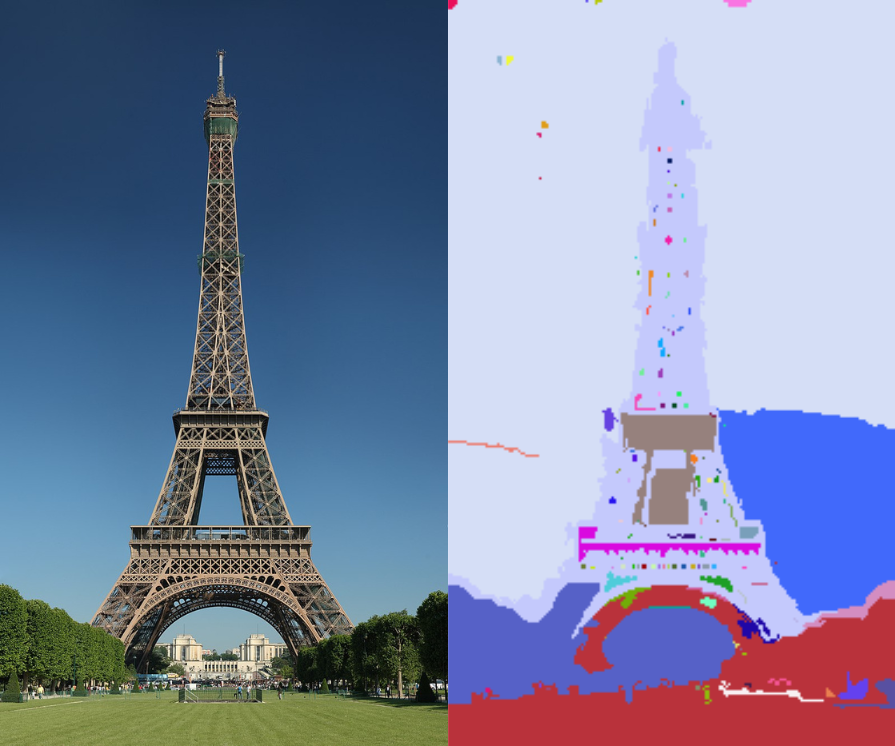
\includegraphics[width=.75\textwidth]{torre_eiffel.png}
\caption{Torre Eiffel}
\label{fig:torre-eiffel}
\end{figure}

\begin{figure}[ht]
\centering
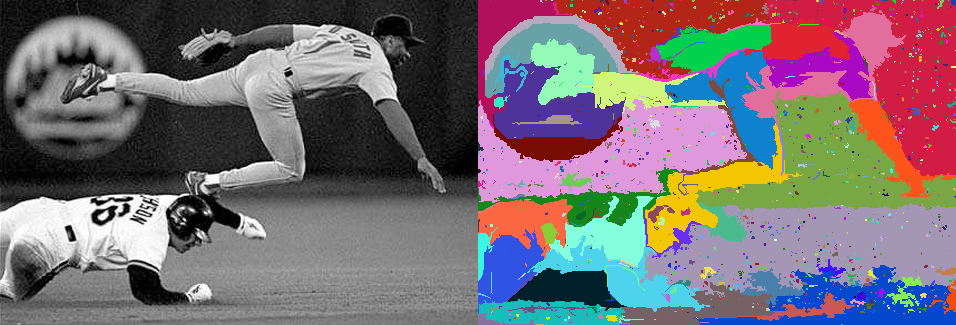
\includegraphics[width=1\textwidth]{jogo_baseball.png}
\caption{Jogo de baseball}
\label{fig:baseball}
\end{figure}

\subsection{Boykov--Funka-Lea}
A partir do algoritmo apresentado na Seção \ref{subsec:abfl}, foi realizada a segmentação de uma imagem. Na Figure \ref{fig:arvore}, apresentamos a imagem original e sua segmentação.

\begin{figure}[ht]
\centering

\includegraphics[width=1\textwidth]{arvore.png}
\caption{Árvore}
\label{fig:arvore}
\end{figure}

\section{Conclusão} \label{sec:conclusion}
Este trabalho implementou e aplicou dois algoritmos distintos para segmentação de imagens baseados em grafos: Felzenszwalb-Huttenlocher e Boykov--Funka-Lea. Cada algoritmo aborda o problema com uma perspectiva única.

Felzenszwalb-Huttenlocher, baseado na identificação de fronteiras entre regiões, demonstrou ser eficiente em imagens com contornos bem definidos e regiões homogêneas (Figure \ref{fig:torre-eiffel} e Figure \ref{fig:baseball}). A escolha do parâmetro $k$ impacta significativamente o resultado. O algoritmo tende a gerar segmentações com regiões mais uniformes em termos de cor.

Boykov--Funka-Lea, que modela a segmentação como minimização de energia por cortes em grafos, demonstrou ser eficaz em segmentar objetos com contornos mais complexos e em imagens com ruído (Figure \ref{fig:arvore}). A utilização de \textit{seeds} permite um controle mais interativo. Em Boykov--Funka-Lea, o parâmetro $\lambda$ controla o balanço entre os termos regionais (t-links) e os termos de fronteira (n-links) na função de energia: valores altos de $\lambda$ resultam em segmentações mais suaves, enquanto valores baixos resultam em segmentações mais detalhadas. O parâmetro $\sigma$, presente na função que calcula o peso dos n-links, controla a sensibilidade às diferenças de intensidade: um $\sigma$ pequeno resulta em segmentações mais detalhadas, e um $\sigma$ grande resulta em segmentações mais suaves. A escolha adequada desses parâmetros, juntamente com a seleção das \textit{seeds}, é crucial para obter bons resultados.

Felzenszwalb-Huttenlocher destaca-se pela simplicidade e eficiência computacional, adequado para aplicações que demandam velocidade e em imagens com características favoráveis. Boykov--Funka-Lea oferece maior precisão e robustez em cenários mais desafiadores, porém com um custo computacional mais elevado e dependência da seleção adequada de \textit{seeds} e dos parâmetros $\lambda$ e $\sigma$.

Como trabalhos futuros, sugere-se a investigação de métodos para aprimorar a escolha automática do parâmetro $k$ no algoritmo de Felzenszwalb-Huttenlocher e a exploração de diferentes estratégias para o cálculo dos pesos das arestas, incluindo a otimização dos parâmetros $\lambda$ e $\sigma$, e a seleção automática de \textit{seeds} no algoritmo de Boykov--Funka-Lea. A aplicação dos algoritmos em diferentes tipos de imagens e a comparação com outros métodos de segmentação também são relevantes.

\section*{Contribuições Individuais}
As contribuições de cada integrante foram:
\begin{itemize}
    \item \textbf{Fábio Antônio C. Andrade:} Implementação do algoritmo Boykov--Funka-Lea. Escrita do artigo.
    \item \textbf{Lucas A. Barros:} Implementação do algoritmo Boykov--Funka-Lea. Escrita do artigo.
    \item \textbf{Pedro M. Lima:} Implementação das estruturas de dados (Grafos, Lista de Arestas e \textit{Union Find}) e dos algoritmos Felzenszwalb-Huttenlocher e Boykov--Funka-Lea.
    \item \textbf{Pedro R. Maia:} Implementação das estruturas de dados (Grafos e Lista de Arestas) e do algoritmo Felzenszwalb-Huttenlocher. Escrita do artigo.
\end{itemize}

\bibliographystyle{sbc}
\bibliography{sbc-template}

\end{document}